% Activate the following line by filling in the right side. If for example the name of the root file is Main.tex, write
% "...root = Main.tex" if the chapter file is in the same directory, and "...root = ../Main.tex" if the chapter is in a subdirectory.
 
%!TEX root =  dissertation.tex

\chapter[Implementation]{Implementation}

In this chapter, I will discuss HemeWeb's project implementation. This will consist on how the HemeLB core container is developed, how it is deployed, and how the web application itself is being implemented.


\section{Deployment}

In addition to have a working prototype available. I also wanted to make sure that the process of deploying the web application is as painless as possible. Therefore, I developed a deployment script for automatically configuring the architecture with minimal manual intervention. The script is made with the help of a configuration management and orchestration tools called ansible (https://www.ansible.com).

The goal of the script are as follow:
1. Provision the required master instance
2. Configure the master instances with the correct security and network settings
3. Configure and Install the HemeWeb correctly
4. Configure and install all the services needed by HemeWeb
5. Provision required compute instance
6. Configure the compute instances with the correct security and network settings
7. Configure the compute instances to run HemeLB core docker container

In the development of the script, I faced few problems in regard of orchestrating the infrastructure. Mainly with regards to cloud vendors having non-similar application programming interface to access or control the resources. This led to some part of the deployment needing manual intervention. One of this part is creating an image from the running instance so the master instance can request a new pre-configured instance instead of configuring from the start.

I developed the script as modular as I can so that it can be refactored easily. I separated the cloud vendor specific instruction into its own folder for each vendor. This part mainly deal with the provisioning, security, and network configurations. The more common part, like installing softwares and services needed, are abstracted into the common scripts that are called by the vendor specific script after provisioning instances are done. With this in mind, I had been able to run the deployment script on three different cloud vendors. They are Google Cloud Platform, Amazon Web Service, and Digital Ocean. After the deployment script is done, the architecture will be ready to run HemeLB simulation on the cloud.

This script is online as part of the codebase that is published on github. It is available on https://github.com/SeiryuZ/HemeWeb/tree/master/deployment .


\section{HemeWeb web application}

This section will discuss the bulk of the work that is developed for the project. The main interface for users to interface with HemeWeb, the web application.  I developed this web application using django web framework for my familiarity with the framework, so I can focus my time on developing the web application.




\subsection{Running a simulation}

The main feature of HemeWeb web application is the ability to run HemeLB simulation. Allowing users without technical know how to run the simulation on command line interface to use web browser to run it. The web application take two input files, geometry file and HemeLB configuration file and store it on the master interface. 

The web interface will then allow users to modify the HemeLB configuration file with an in-browser text editor and also configure the job execution like compute instance count, compute instance type, and the HemeLB core container to use. After the configuration is done, the job will be queued into a queue system which are based on a redis Pub/Sub mechanism. 

An asynchronous workers (Different from the web application workers) will then pick up the queued up job. The worker will run an ansible script to startup correct amount of compute unit from the cloud vendor. For this project, amazon web service is the only available cloud vendors. The compute unit will be started up from the state after the configuration on the deployment part, so it will not waste too much time to configure the base image. However, this is not yet ready to run the HemeLB simulation. What the script will do next is to reconfigure the compute unit more, like reconfiguring docker service to point to the correct master address, mounting the remote file system containing the input files, pull the correct HemeLB core container from docker hub, and run the container.

After all the reconfiguration processes are done, the master's asynchronous worker will then fire an mpi job for HemeLB with the correct parameters. HemeLB simulation will run and produce output which will be written to the shared folder with the master instance. The compute instances will be terminated after the simulation is done.

Outputs of the simulations are then made available for the users to be downloaded via the web interface.

These features are part of the original scope of the web application as I planned on my proposal \citep{Steven:2016aa}. However, I extended the web application so that it can handle more cases. The first thing I added were the ability to handle the pre-processing of the input files. The input files that are used by the HemeLB simulation are generated from a geometry generation step that are done before the simulation. This geometry generation step took different input files, a geometry file (.stl) and a profile file (.pr2) to generate the input that HemeLB simulation can parse. 

The way I implement the pre-processing stuff is to add another form for user to add input files to create new job. It receive the .stl and .pr2 file, save them, and queue up an asynchronous job that will pre-process these input into the correct files that will be feed into the HemeLB simulation configuration part.

Also, I added post-processing feature to the web application. The output files generated by the HemeLB simulation are effective to write in parallel. However, these files are not directly viewable by software like VTK viewer. These files need further post-processing, this is where the post-processing step is introduced in HemeWeb. I added the post-processing step, piping the outputted files into two python scripts, into the asynchronous worker. So after the HemeLB simulation step is done, it has an extra responsibility to run the post processing step on the master interface. The outputted files then will be packaged with the original output for download by the user.


\subsection{Reproducing a simulation}


\subsection{Persistence}


\subsection{HemeWeb workflow}

\vspace{1cm}

\noindent%
\begin{minipage}{\linewidth}% to keep image and caption on one page
\makebox[\linewidth]{
  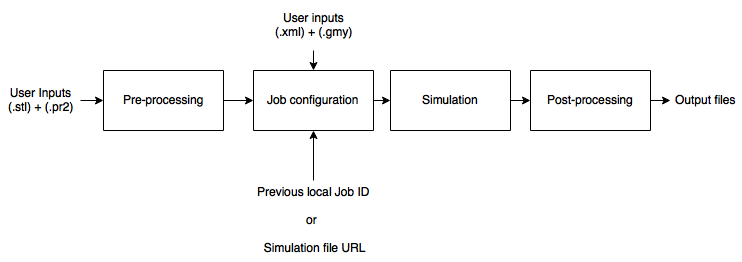
\includegraphics[keepaspectratio=true,scale=0.5]{../resources/images/implementation.png}
 }
\captionof{figure}{HemeWeb flow}\label{fig:hemeweb-implementation}%      only if needed  
\end{minipage}

\vspace{1cm}

Figure \ref{fig:hemeweb-implementation} illustrate how the HemeWeb web application works. it consists of mainly 4 core activity that will be discussed in details in the following section.

\subsubsection{Pre-processing}

HemeWeb handle pre-processing of inputs that are needed so that HemeLB simulation can parse the files. User provide a geometry file (.stl) and a profile file (.pr2) to the web application. HemeWeb will then create a job instance with these two files, save them locally on master instances and queue the pre-processing job.

The asynchronous worker on master instance will then pick up the job whenever they are free. It will run the pre-processing python script to generate the geometry files and HemeLB configuration file. These files will then be saved on the master instance, and HemeWeb will track these files by recording the path to these files on the job instance. Now the job instance is ready for the next step. of the workflow.

\subsubsection{Job configuration}

In this step, HemeWeb application will take a job instance with correctly set geometry file (.gmy) and HemeLB configuration (.xml). However, there are multiple ways that HemeWeb can get this correctly set job instance. As illustrated on Figure \ref{fig:hemeweb-implementation} , there are 4 possible entry points for this step. They are:

\begin{itemize}
    \item \textbf{From the post-processing step.}
    	These files are generated from the previous pre-processing step. The job instance is directly used in this step
    
    \item \textbf{User's provided geometry and configuration file.}
    	User have pre-processed their own file locally, or have their own geometry and configuration files available. HemeWeb will create a new job instance, save both files and keep them tracked with the job instance.
	
    \item \textbf{User's provided previous job ID.}
    	There are two possible case when user specify previous job ID. First, the previous job is available locally on the HemeWeb instance. Second, the previous job is cached on the persistent storage on the cloud vendor and are not available locally. HemeWeb will download the previous file from the persistent storage if it is not available locally. It will then create a new job instance that copy the previous job's geometry file and configuration file to be used for further configuration.
    
    \item \textbf{User's provided simulation file URL.}
    	The last alternative is for user to provide the simulation file URL. Simulation files are uploaded to a persistent storage at the end of the workflow. These files, if made public, can be used by other instance of HemeWeb to download the simulation files and use it as a basis to create a new job instance. The way the system work is the same as using previous job ID, but its source is not its own persistent storage, but other people's simulation files.

\end{itemize}


After the job instance is created from one of the four way possible discussed above, HemeWeb will then ask users for the job configuration. This entails on configuring how many instances should be started, what are the type of the instance, and the hemelb-core container version.  After configuring all these parameters, then the user can queue the job into the queue system.	



\subsubsection{HemeLB simulation}

Once job instance are queued into the simulation queue, free asynchronous workers will pop the queue and run the job. The worker will start up the configured amount and type of server instance from the cloud provider. These instances will then be further reconfigured by an ansible script so that it points to the correct master instance address. Next, input files are shared via Networked File System(NFS), the compute units will mount the input folders to their instance. 

HemeLB core container will be pulled from docker hub in the next step. This step will skip the download if the container asked are already cached in the image for compute unit which are prepared on the deployment part. After all of these are done, then the simulation can finally begin. Master node will issue an mpi command to be run by the leader of compute nodes. The leader of compute node then will run this mpi command in the docker container. This command will be run on multiple compute node if it is configured as such in the previous steps. 

The HemeLB simulation will run until outputs are produced. The output will be written back to the correct output folder in the shared folder. This means that the master instance will have access to the outputs file and can do further processing. This step ends with the termination of the instances.


\subsubsection{Post-processing}

After HemeLB simulation is done, HemeWeb web app will do some post-processing steps to make sure the output files can be viewed easily. The output from HemeLB simulation is structured in such a way that makes it efficient to write in parallel. However, these output cannot be viewed by visualization system like Paraview. What HemeWeb will do is to pipe the output to two scripts that will format the output into a format that can be understood by paraview.


However, the post-processing steps are not done until converting the output. There are further steps that HemeWeb took to make sure that the simulation files, configurations, and results are preserverd. HemeWeb will package the job directory, compressed it, and upload it into persistent storage that cloud vendors provide. As the time of writing, HemeWeb only support amazon S3. The simulation file are uploaded to this storage and made available for public for other HemeWeb instance to use. Also, with the job files persisted on persistent storage. The next HemeWeb instance deployed can take advantage of these files that it can download them as previous job available.



\subsection{Job directory structure}

HemeWeb structure each job's files and configurations into its own folder. I will discuss how it is structure to provide clearer picture on how the application package and work with the job's files.

\begin{lstlisting}
<UPLOAD_FOLDER_DIR>/<JOB_ID>
<UPLOAD_FOLDER_DIR>/<JOB_ID>/inputs/*
<UPLOAD_FOLDER_DIR>/<JOB_ID>/logs/*
<UPLOAD_FOLDER_DIR>/<JOB_ID>/outputs/*
<UPLOAD_FOLDER_DIR>/<JOB_ID>/metadata
\end{lstlisting}

HemeWeb installation can change the upload folder directory as the basis of all job's folder will be located.  Job ID will be generated by the web application using UUID4 scheme, so ID's generated by different instances of HemeWeb should theoretically have really low chance of clashing. This is also why adding previous job to the HemeWeb instance is not problematic, because using auto increment ID will be a problem for multiple installation.

Next, we have the inputs folder inside the job folder. This is where all the inputs and configurations are stored by the web application. There's also logs folder, where the job stdout, stderr, and HemeLB logs are stored. The web application will read from this folder and make it available on the web interface. Outputs folder will be used by the HemeLB simulation to output files on this folder. One final file is the metadata file. This file is used by the web application to store the state of the job. The job is pickled into this metadata file so when it is downloaded, the web application can unpickle the state of the job instance and it is preserved, ready to be used for another simulation.




\subsection{Challenge}

One problem that I faced on developing the web application is that currently, it is developed mainly for the use on amazon web service (AWS). Due to the limited time for the development, I haven't been able to develop the features on multiple cloud vendors. The features like, automatically uploading simulation file and restoring previous simulations, are tied in the code to the amazon infrastructure. It should be possible to abstract these features to handle multiple cloud vendors given more time.


